\documentclass[18pt]{beamer}
\usepackage[T1]{fontenc}
\usepackage[protrusion=true,expansion=true]{microtype}
%usepackage[minionint,mathlf]{MinionPro}
\usepackage[sc,osf]{mathpazo}
%\renewcommand{\sfdefault}{Myriad-LF}

\usepackage{textcomp}
\usepackage{graphicx}
\usepackage{semantic}

\usetheme{default}
\usefonttheme{professionalfonts}
%\usefonttheme[]{structuresmallcapsserif}
\begin{document}

\frame{
  \begin{center}
    Formalization of JANUS\\
    \emph{or}\\
    ``Explaining your proof to the machine''\\
    (Work in progress)
  \end{center}
}

\frame{
  \begin{center}
    The Great Human Grid Computer
  \end{center}
}

\frame{
  \begin{center}
    \large{Goals:}\\
    \begin{itemize}
    \item Simplicity
    \item It is in the details!
    \item Understanding the domain.
    \end{itemize}
  \end{center}
}

% \frame{
%   \begin{center}
%     Coq\\
%     \begin{itemize}
%     \item Proof verification
%     \item Proof assistance
%     \item Automated Theorem Proving
%     \end{itemize}
%   \end{center}
% }

\frame{
  \begin{center}
    Curry-Howard correspondance:\\
    \begin{tabular}{lll}
      Logic & & PL\\
      \hline \hline
      Proposition & $\simeq$ & Type \\
      Proof       & $\simeq$ & Program\\
      \hline
    \end{tabular}
  \end{center}
}

\frame{
  \begin{center}
    Coq:\\
    ML + Proven termination\\
    +\\
    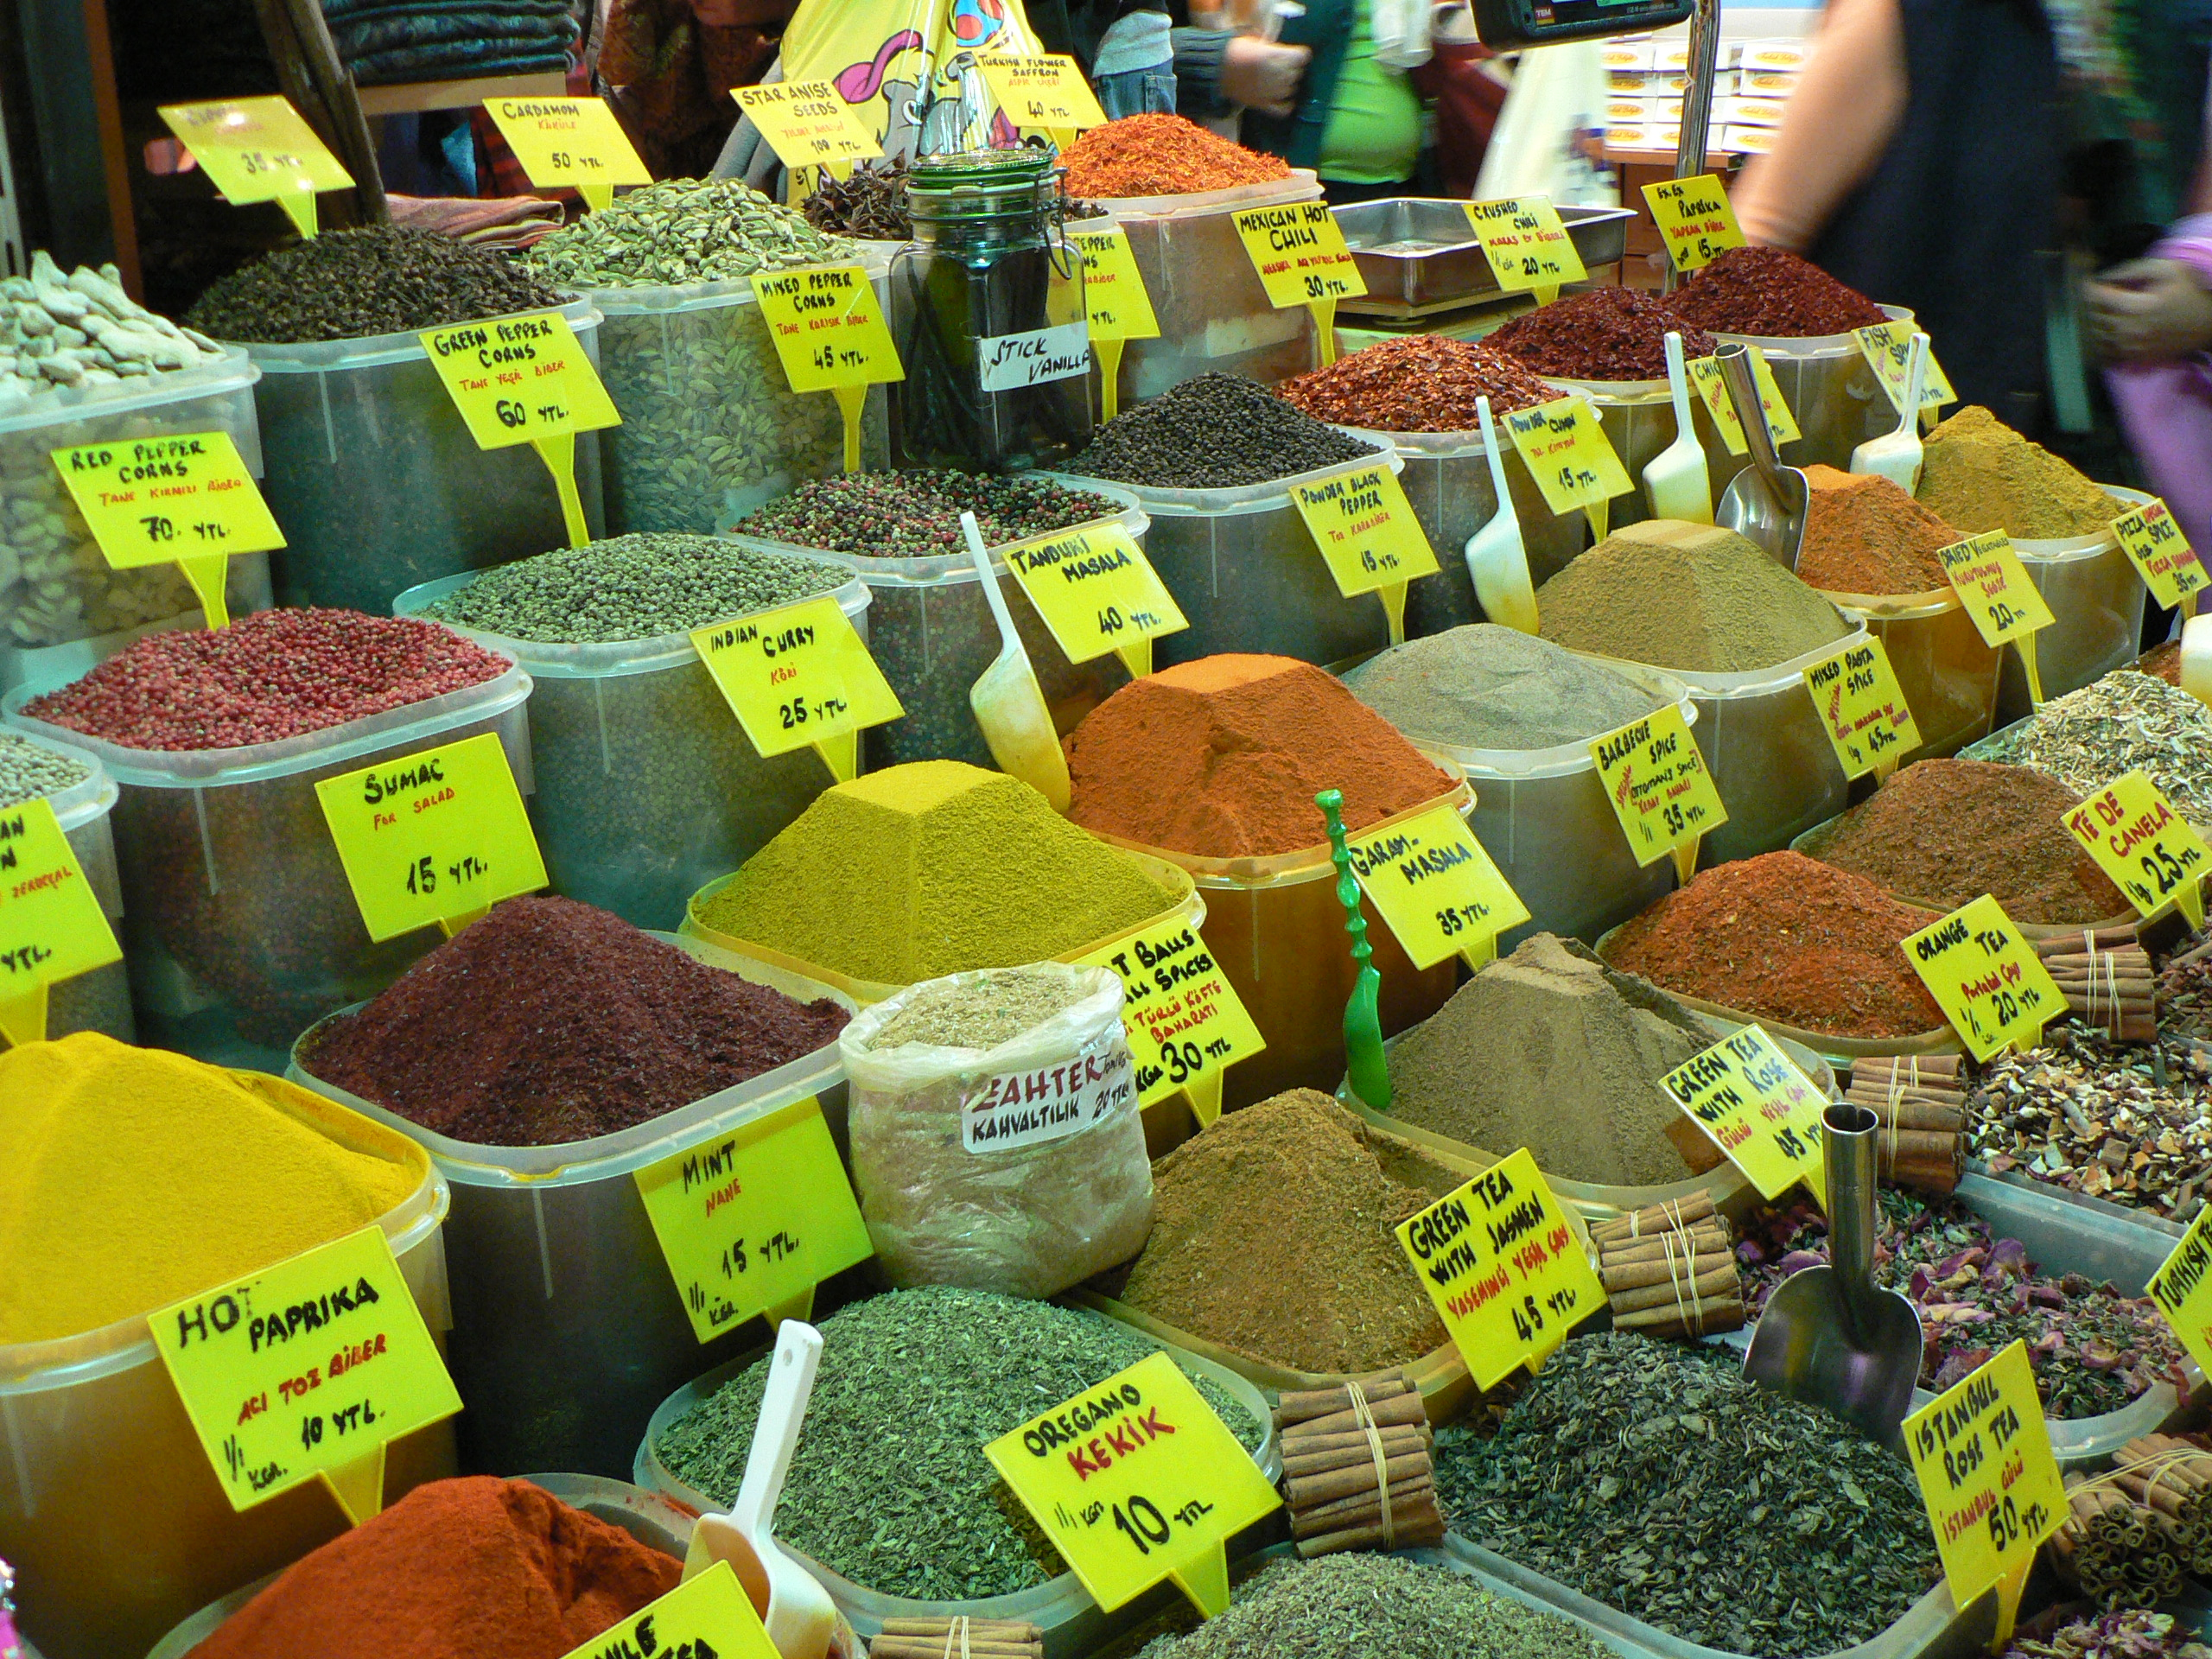
\includegraphics[width=200px]{Kruiden}
  \end{center}
}

\frame{
  \begin{center}
    Formalizing\\
    JANUS\\
    (Work in progress!)
  \end{center}
}

\frame{
  \begin{center}
    32-bit number representation:\\
    integer $z \in \mathbb{Z}$, and\\
    A proof of $0 \leq z < 2^{32}$.\\
    Key Lemma:\\
    $\forall z \in \mathbb{Z}, \quad 0 \leq z \mod 2^{32} < 2^{32}$
  \end{center}
}

\frame{
  \begin{center}
    Store representation:\\
    1st attempt:\\
    $\sigma \colon \mathrm{Var} \to \mathrm{w32}$\\
    \small{\texttt{Definition empty (\_ : var) := 0.}}\\
    2nd attempt:\\
    $\sigma \colon \mathrm{Var} \to \mathrm{w32}_{\perp}$\\
    \small{\texttt{Definition empty (\_ : var) := None.}}
  \end{center}
}

\frame{
  \begin{center}
    Expressions:\\
    $\sigma |- e => n$\\
    Inputs: $\sigma$ and $e$, outputs: $n$.\\
    Don't need a relation!\\
    $denoteExp \colon \mathrm{store} \to \mathrm{exp} \to \mathrm{w32}$
  \end{center}
}

\frame{
  \begin{center}
    Statement loops:\\
    \begin{itemize}
    \item The PEPM 2007 paper uses a global property on loops.
    \item No local determinism (inversion property).
    \item Hard to prove in Coq.
    \item Solution: Rewrite semantics.
    \end{itemize}
  \end{center}
}

\frame{
  \begin{center}
    Statement assignments:\\
    $x \; +\!\!= e$
    \begin{itemize}
    \item $x$ must not occur in $e$. No formalization in the PEPM2007
      paper.
    \item 1st attempt: Drive a syntactic check (static semantics)
    \item 2nd attempt: Implement store hiding!
    \end{itemize}
  \end{center}
}

\frame{
  \begin{center}
    Current status:
    \begin{itemize}
    \item Working towards a proof of forward/backward determinism mutually.
    \item Need properties on stores to do it.
    \item No arrays yet.
    \item Extensionality may come in handy:
    \end{itemize}
    $\forall x, \quad f \; x = g \; x => f = g$
  \end{center}
}

\frame{
  \begin{center}
    But how does it look in the real world?\\
    ProofGeneral, an emacs environment for proof assistants:\\
    
\includegraphics[width=100px]{ProofGeneral}
  \end{center}
}


\end{document}

%%% Local Variables: 
%%% mode: latex
%%% TeX-master: t
%%% End: 

%%% Local Variables: 
%%% mode: latex
%%% TeX-master: t
%%% End: 
